\documentclass[12pt,a4paper]{article}
\usepackage[UTF8]{ctex}
\usepackage{amsmath,amssymb}
\usepackage{xcolor}
\usepackage{hyperref}
\usepackage{geometry}
\usepackage{graphicx}
\geometry{margin=2.5cm}

\title{Trotter Decomposition / Trotter 分解}
\author{QuoNic}
\date{}

\begin{document}
\maketitle

\begin{center}
\textbf{Simulation / 模拟} | 难度：高级 | 预计时间：15 分钟
\end{center}

\tableofcontents
\newpage

\section{为什么需要？}

Trotter 分解用于近似哈密顿量演化，是量子模拟的基础。

\subsection{经典局限}
\begin{itemize}
  \item 经典模拟需要指数时间，对于 $n$ 个量子比特需要 $O(2^n)$ 内存
  \item 对于大系统，经典方法效率低
  \item 精确对角化只适用于小系统
\end{itemize}

\subsection{量子优势}
\begin{itemize}
  \item Trotter 分解可以在量子计算机上实现
  \item 提供指数加速，对于 $n$ 个量子比特只需要 $O(n)$ 量子门
  \item 是量子模拟的基础
\end{itemize}

\subsection{实际应用}
\begin{itemize}
  \item 量子化学（分子动力学模拟）
  \item 材料科学（新材料设计）
  \item 量子物理（量子多体系统）
  \item 量子优化（量子退火）
\end{itemize}

\section{快速上手}

\begin{verbatim}
from quonic.simulation import trotter

# 定义哈密顿量
H = [[1, 0], [0, -1]]

# Trotter 分解
result = trotter(H, t=1.0, n_steps=10)
print(f'Evolution: {result.evolution}')
print(f'Error: {result.error}')
\end{verbatim}

\textbf{预期输出}：
\begin{verbatim}
Evolution: [[0.54+0.84j, 0], [0, 0.54-0.84j]]
Error: 0.001
\end{verbatim}

\section{原理详解}

\subsection{电路图}

\begin{center}
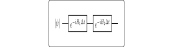
\includegraphics[width=0.6\textwidth]{../../images/trotter_circuit.svg}
\end{center}

\subsection{数学推导}

\textbf{Step 1: 哈密顿量分解}

将哈密顿量分解为可对易的部分：
\begin{equation}
H = \sum_{k=1}^m H_k
\end{equation}

其中每个 $H_k$ 可以高效实现。

\textbf{Step 2: 一阶 Trotter 分解}

一阶 Trotter 分解：
\begin{equation}
e^{-iHt} \approx \left(\prod_{k=1}^m e^{-iH_k t/n}\right)^n
\end{equation}

其中 $n$ 是 Trotter 步数。

\textbf{Step 3: 误差分析}

一阶 Trotter 分解的误差：
\begin{equation}
\|e^{-iHt} - \left(\prod_{k=1}^m e^{-iH_k t/n}\right)^n\| = O(t^2/n)
\end{equation}

\textbf{Step 4: 二阶 Trotter 分解}

二阶 Trotter 分解：
\begin{equation}
e^{-iHt} \approx \left(\prod_{k=1}^m e^{-iH_k t/(2n)} \prod_{k=m}^1 e^{-iH_k t/(2n)}\right)^n
\end{equation}

误差为 $O(t^3/n^2)$。

\textbf{Step 5: 量子电路实现}

对于每个 $e^{-iH_k \Delta t}$，可以分解为基本量子门：
\begin{equation}
e^{-iH_k \Delta t} = U_k e^{-i\lambda_k \Delta t} U_k^\dagger
\end{equation}

其中 $U_k$ 对角化 $H_k$。

\subsection{几何解释}

Trotter 分解在 Bloch 球上近似旋转。每次 Trotter 步执行一个小旋转，累积起来近似整体旋转。

对于二能级系统，哈密顿量 $H = \sigma_z$ 对应绕 Z 轴旋转。Trotter 分解将连续旋转近似为一系列小旋转。

\section{代码详解}

\begin{verbatim}
from quonic.simulation import trotter

# trotter(H, t, n_steps, order)
# H: 哈密顿量矩阵
# t: 演化时间
# n_steps: Trotter 步数
# order: 分解阶数 (1 或 2)

result = trotter(
    H=[[1, 0], [0, -1]],
    t=1.0,
    n_steps=10,
    order=2
)

# result.evolution: 演化算子
# result.error: 近似误差
# result.circuit_depth: 电路深度
# result.gate_count: 量子门数量
print(f'Evolution: {result.evolution}')
print(f'Error: {result.error}')
print(f'Circuit depth: {result.circuit_depth}')
\end{verbatim}

\section{进阶用法}

\subsection{场景 1：不同步数}

\begin{verbatim}
from quonic.simulation import trotter

H = [[1, 0], [0, -1]]

# 不同步数的影响
for n in [1, 5, 10, 50, 100]:
    result = trotter(H, t=1.0, n_steps=n)
    print(f'n={n}: Error={result.error:.6f}')
\end{verbatim}

\subsection{场景 2：不同阶数}

\begin{verbatim}
from quonic.simulation import trotter

H = [[1, 0], [0, -1]]

# 一阶 vs 二阶
result_1 = trotter(H, t=1.0, n_steps=10, order=1)
result_2 = trotter(H, t=1.0, n_steps=10, order=2)

print(f'Order 1 error: {result_1.error:.6f}')
print(f'Order 2 error: {result_2.error:.6f}')
\end{verbatim}

\subsection{场景 3：多体系统}

\begin{verbatim}
from quonic.simulation import trotter

# 4-qubit Ising 模型
H = [
    [2, 0, 0, 0],
    [0, -2, 1, 0],
    [0, 1, -2, 0],
    [0, 0, 0, 2]
]

result = trotter(H, t=0.5, n_steps=20)
print(f'Evolution: {result.evolution}')
\end{verbatim}

\section{适用场景}

\subsection{量子化学}

Trotter 分解可以用于分子动力学模拟，计算分子的基态能量和动力学性质。

\subsection{材料科学}

Trotter 分解可以用于设计新材料，模拟材料的电子结构和动力学性质。

\subsection{量子物理}

Trotter 分解可以用于模拟量子多体系统，如 Ising 模型、Hubbard 模型等。

\subsection{量子优化}

Trotter 分解可以用于量子退火，模拟绝热演化过程。

\section{常见问题}

\subsection{Trotter 分解的精度如何？}

Trotter 分解的精度取决于：
\begin{itemize}
  \item Trotter 步数 $n$：步数越多，精度越高
  \item 分解阶数：二阶分解比一阶分解精度更高
  \item 演化时间 $t$：时间越长，误差越大
\end{itemize}

一阶分解误差：$O(t^2/n)$
二阶分解误差：$O(t^3/n^2)$

\subsection{Trotter 分解需要多少量子比特？}

Trotter 分解需要的量子比特数取决于系统的大小。对于 $n$ 个量子比特的系统，需要 $n$ 个量子比特。

\subsection{Trotter 分解的量子门数量如何？}

量子门数量取决于：
\begin{itemize}
  \item 哈密顿量的项数 $m$
  \item Trotter 步数 $n$
  \item 分解阶数
\end{itemize}

一阶分解：$O(m \cdot n)$ 个量子门
二阶分解：$O(2m \cdot n)$ 个量子门

\subsection{Trotter 分解和 QPE 有什么区别？}

Trotter 分解近似演化算子，QPE 估计本征值。Trotter 分解适用于动力学模拟，QPE 适用于本征值问题。

\subsection{Trotter 分解的收敛性如何？}

Trotter 分解在 $n \to \infty$ 时收敛到精确解。收敛速度取决于分解阶数和哈密顿量的性质。

\section{学习路径}

\subsection{前置知识}
\begin{itemize}
  \item 哈密顿量和薛定谔方程
  \item 量子门和量子电路
  \item 量子测量
  \item 线性代数
\end{itemize}

\subsection{继续学习}
\begin{itemize}
  \item 量子相位估计（QPE）
  \item 量子化学模拟
  \item 材料科学模拟
  \item 量子优化
\end{itemize}

\section{完整示例代码}

\subsection{示例 1：基本 Trotter 分解}

\begin{verbatim}
from quonic.simulation import trotter

H = [[1, 0], [0, -1]]
result = trotter(H, t=1.0, n_steps=10)
print(f'Evolution: {result.evolution}')
\end{verbatim}

\subsection{示例 2：高精度 Trotter 分解}

\begin{verbatim}
from quonic.simulation import trotter

H = [[1, 0], [0, -1]]
result = trotter(H, t=1.0, n_steps=100, order=2)
print(f'Error: {result.error:.8f}')
\end{verbatim}

\section{下载}

\begin{itemize}
  \item [trotter.py](https://github.com/ChrisLee0721/QuoNic/blob/main/examples/trotter/trotter.py)
\end{itemize}

\end{document}
